\section{Verification and analysis}
\label{sec:verification}
In this section, we present the verification of our SASS method as described in
\Cref{sec:method}. First we qualitatively verify that SASS is sound by
comparing the resulting segmentation to the original tomography and defining an
artificial ground truth. Then we quantitatively verify the SASS method by
generating synthetic data, evaluating it on the created ground truth, and
comparing the results to other existing methods. Finally, we analyze the
segmented data to study the blood vessel network in the bone region and produce
statistics on the tissue-to-implant contact.

\subsection{Qualitative evaluation}

Since the SRµCT tomograms are clear enough that humans can distinguish between
blood vessels and bone, as our mammalian visual cortex automatically corrects
for the distortion effects, we can verify the success of the automatic
classification. We can compare the automatic classification with the manual
classification of the histological microscopy. A larger quantitative study is
planned that analyses the full data set against recently conducted histological
microscopy taken from the same biopsies.

\Cref{fig:histology-comparison1} and \Cref{fig:histology-comparison2} show the
same 2D slices as were shown in \Cref{fig:3viewsample} and \Cref{fig:slices},
allowing us to visually inspect them side by side. The voxels are colored
according to the segmentation confidence, with the degree of red being
proportional to the modeled probability $\Pof{0}{v,\fval}$ and the degree of
yellow being proportional to $\Pof{1}{v,\fval}$. Grey voxels indicate low model
probabilities of both: either due to the voxel belonging to another material or
simply low computed confidence of the model.  By comparing the images in
\Cref{fig:histology-comparison1} and \Cref{fig:histology-comparison2}, we see
that the global thresholding (top right) fails to capture the soft tissue
close to the implant, which further confirms the need for a more sophisticated
method. Looking at the adaptive Otsu segmentation (bottom right), we see that it better
captures the soft tissue close to the implant, but still fails even closer to
the implant. SASS (bottom left) captures the soft tissue close to the
implant, while still ensuring a good segmenting in previously well segmented
regions.

\begin{figure*}
  \centering
    \begin{subfigure}{0.5\textwidth}
      \centering
      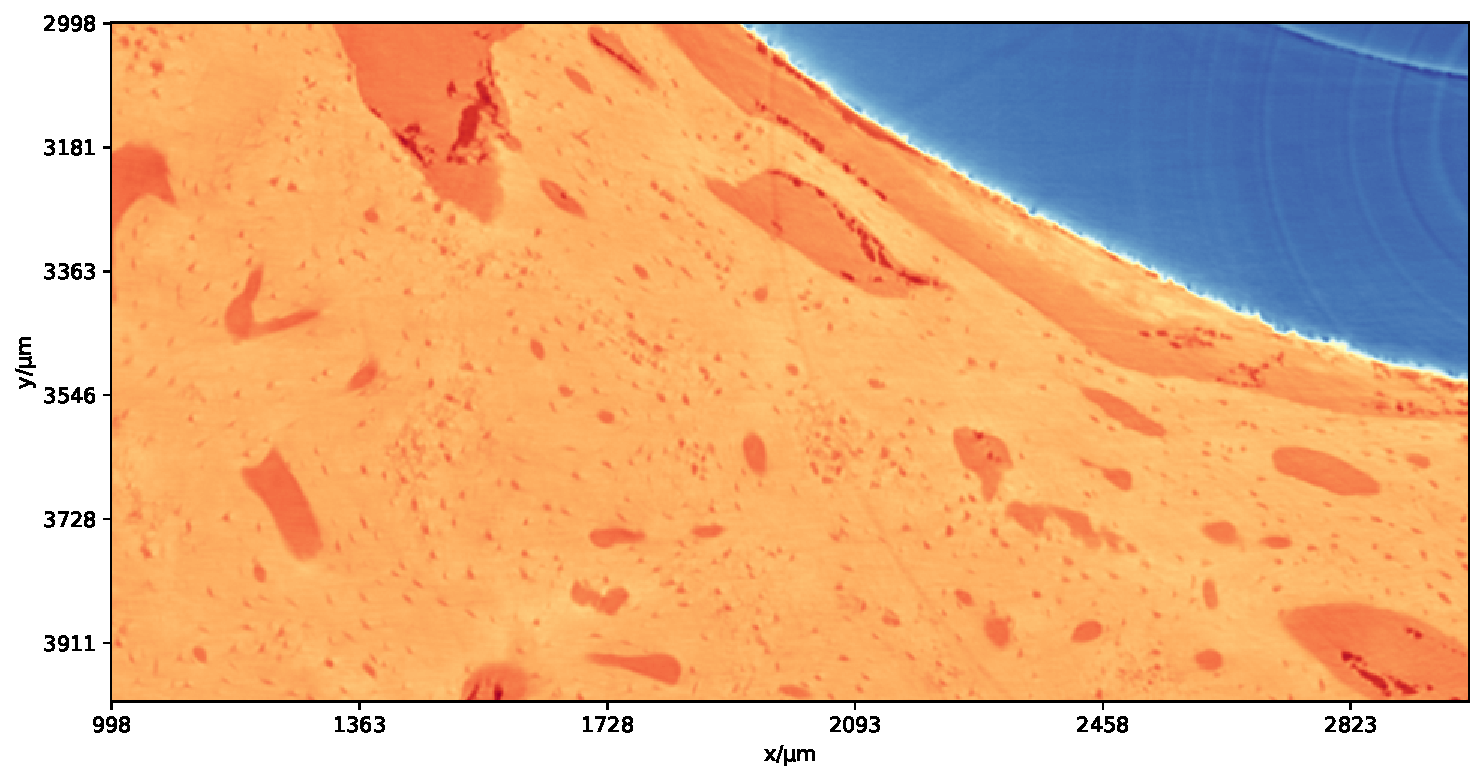
\includegraphics[width=\linewidth]{generated/770c_pag_segmented_yx_raw.pdf}
      \caption{Tomographic slice}
    \end{subfigure}%
    \begin{subfigure}{0.5\textwidth}
      \centering
      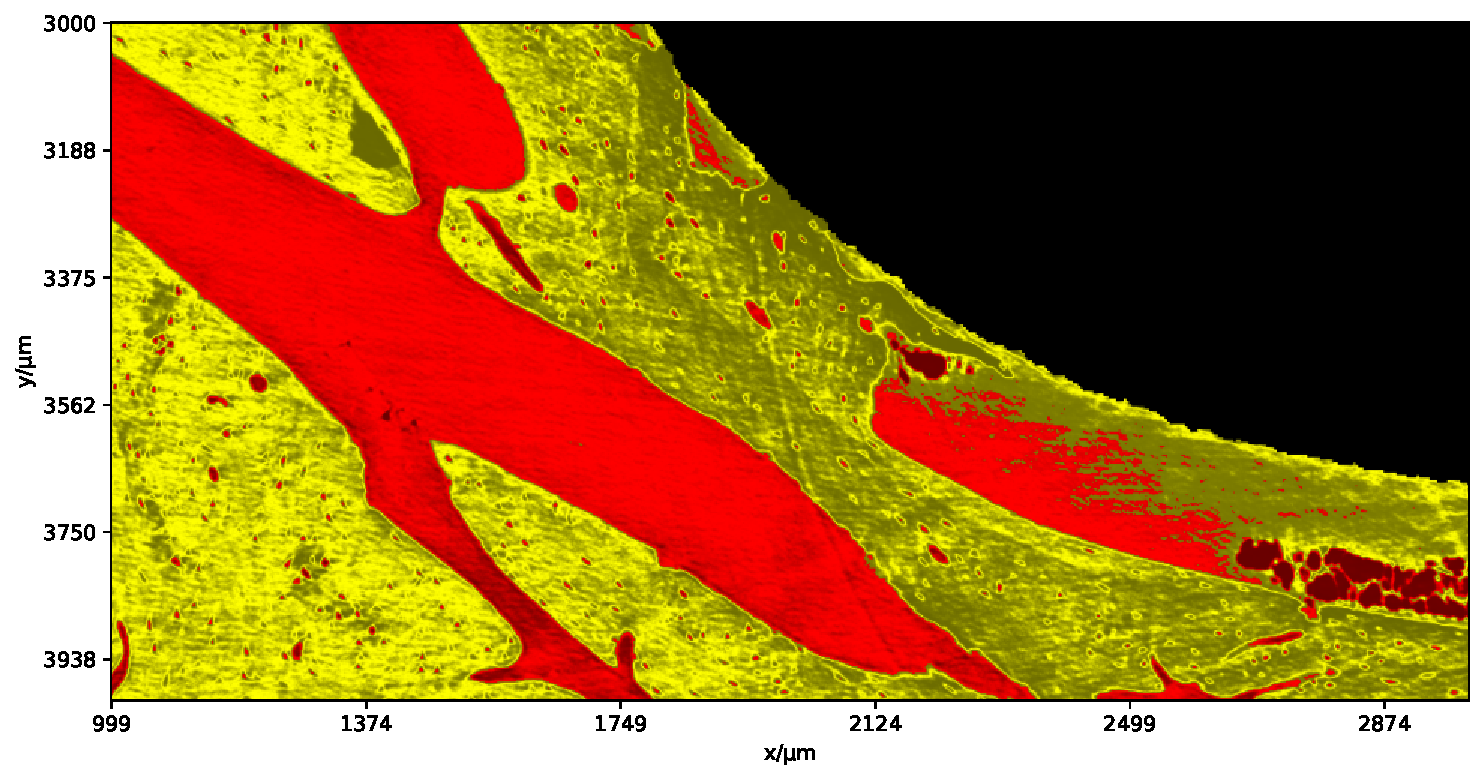
\includegraphics[width=\linewidth]{generated/770c_pag_global_yx.pdf}
      \caption{Global threshold}
    \end{subfigure}
    \\
    \begin{subfigure}{0.5\textwidth}
      \centering
      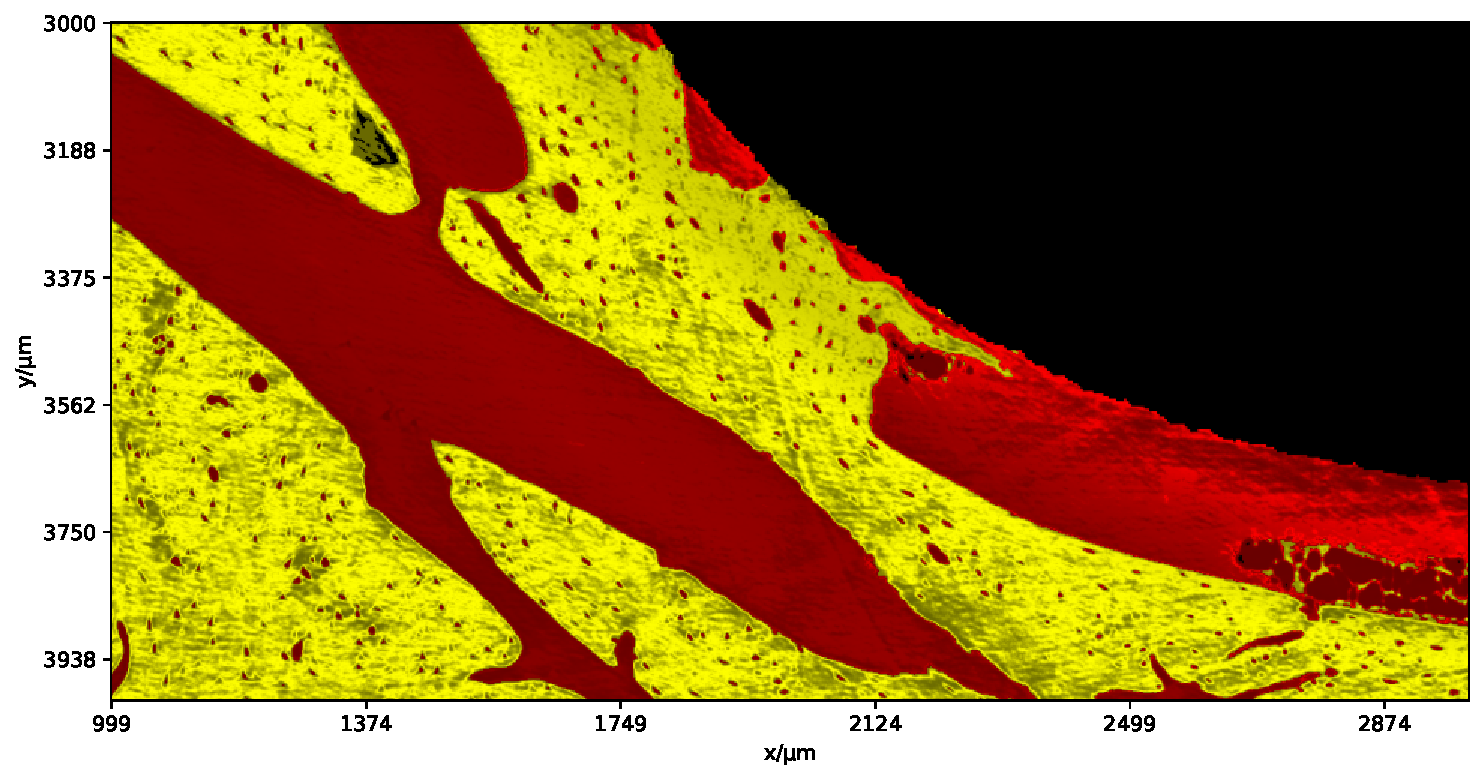
\includegraphics[width=\linewidth]{generated/770c_pag_segmented_yx_colored.pdf}
      \caption{SASS}
    \end{subfigure}%
    \begin{subfigure}{0.5\textwidth}
      \centering
      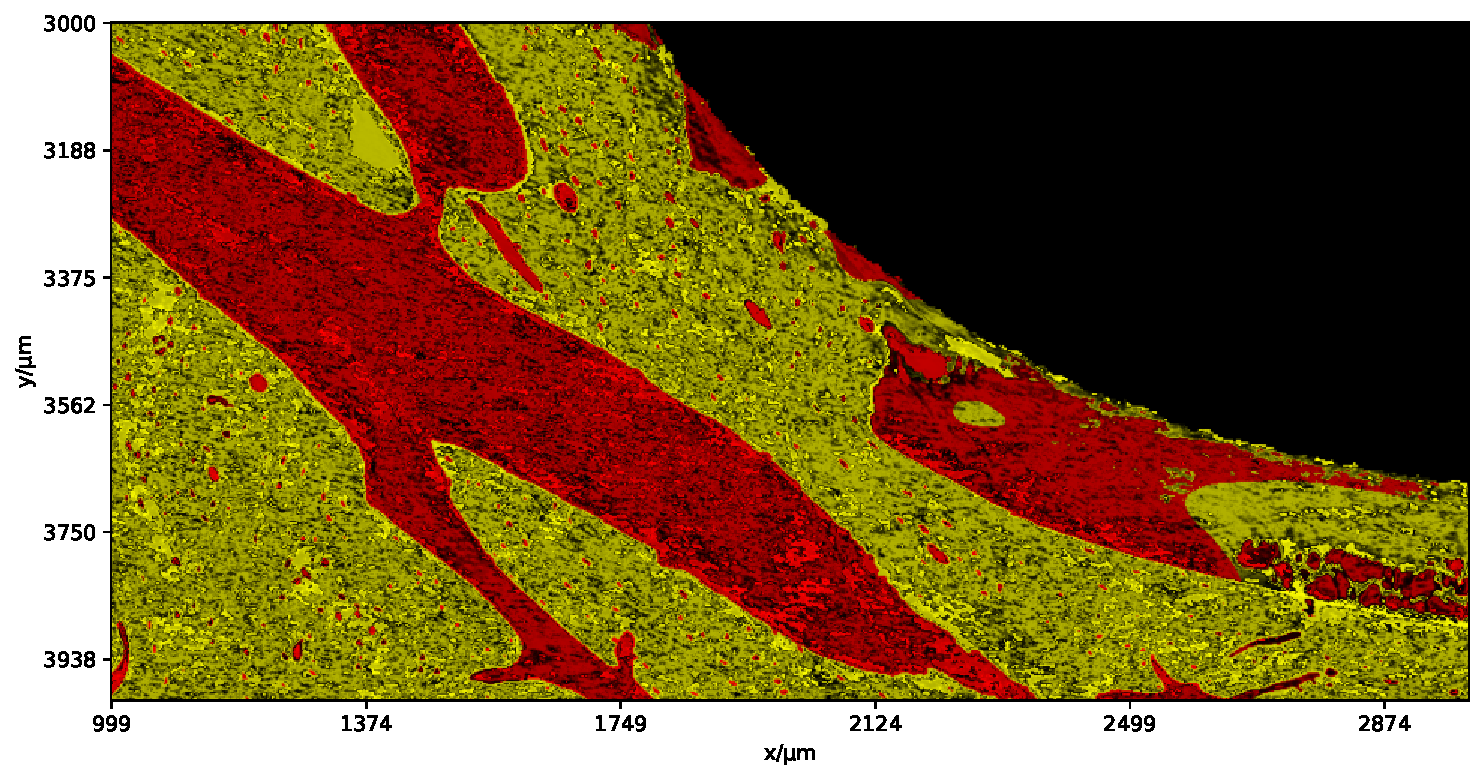
\includegraphics[width=\linewidth]{generated/770c_pag_global_yx_otsu.pdf}
      \caption{Adaptive Otsu}
    \end{subfigure}
  \caption{
	  YX-slices of the original tomography, Adaptive Otsu segmentation, SASS,
	  and global threshold segmentation. For SASS, the voxels
	  are colored according to the modeled probability functions $P(m\vert
	  v,\fval)$ between 0 and 1: completely red voxels have $P(m=0\vert
	  v,\fval) = 1$, completely yellow voxels have $P(m=1\vert v,\fval)\ =
	  1$, and uncertain voxels become progressively gray. Notice how the
	  global threshold fails to segment a large region of blood vessel in
	  the bottom right, leaving a clear streak pattern. This is due to the
	  shifted numerical values from the streak effects mentioned in
	  \Cref{fig:slices}.
    }
    \label{fig:histology-comparison1}
\end{figure*}

\begin{figure*}
  \centering
    \begin{subfigure}{0.5\textwidth}
      \centering
      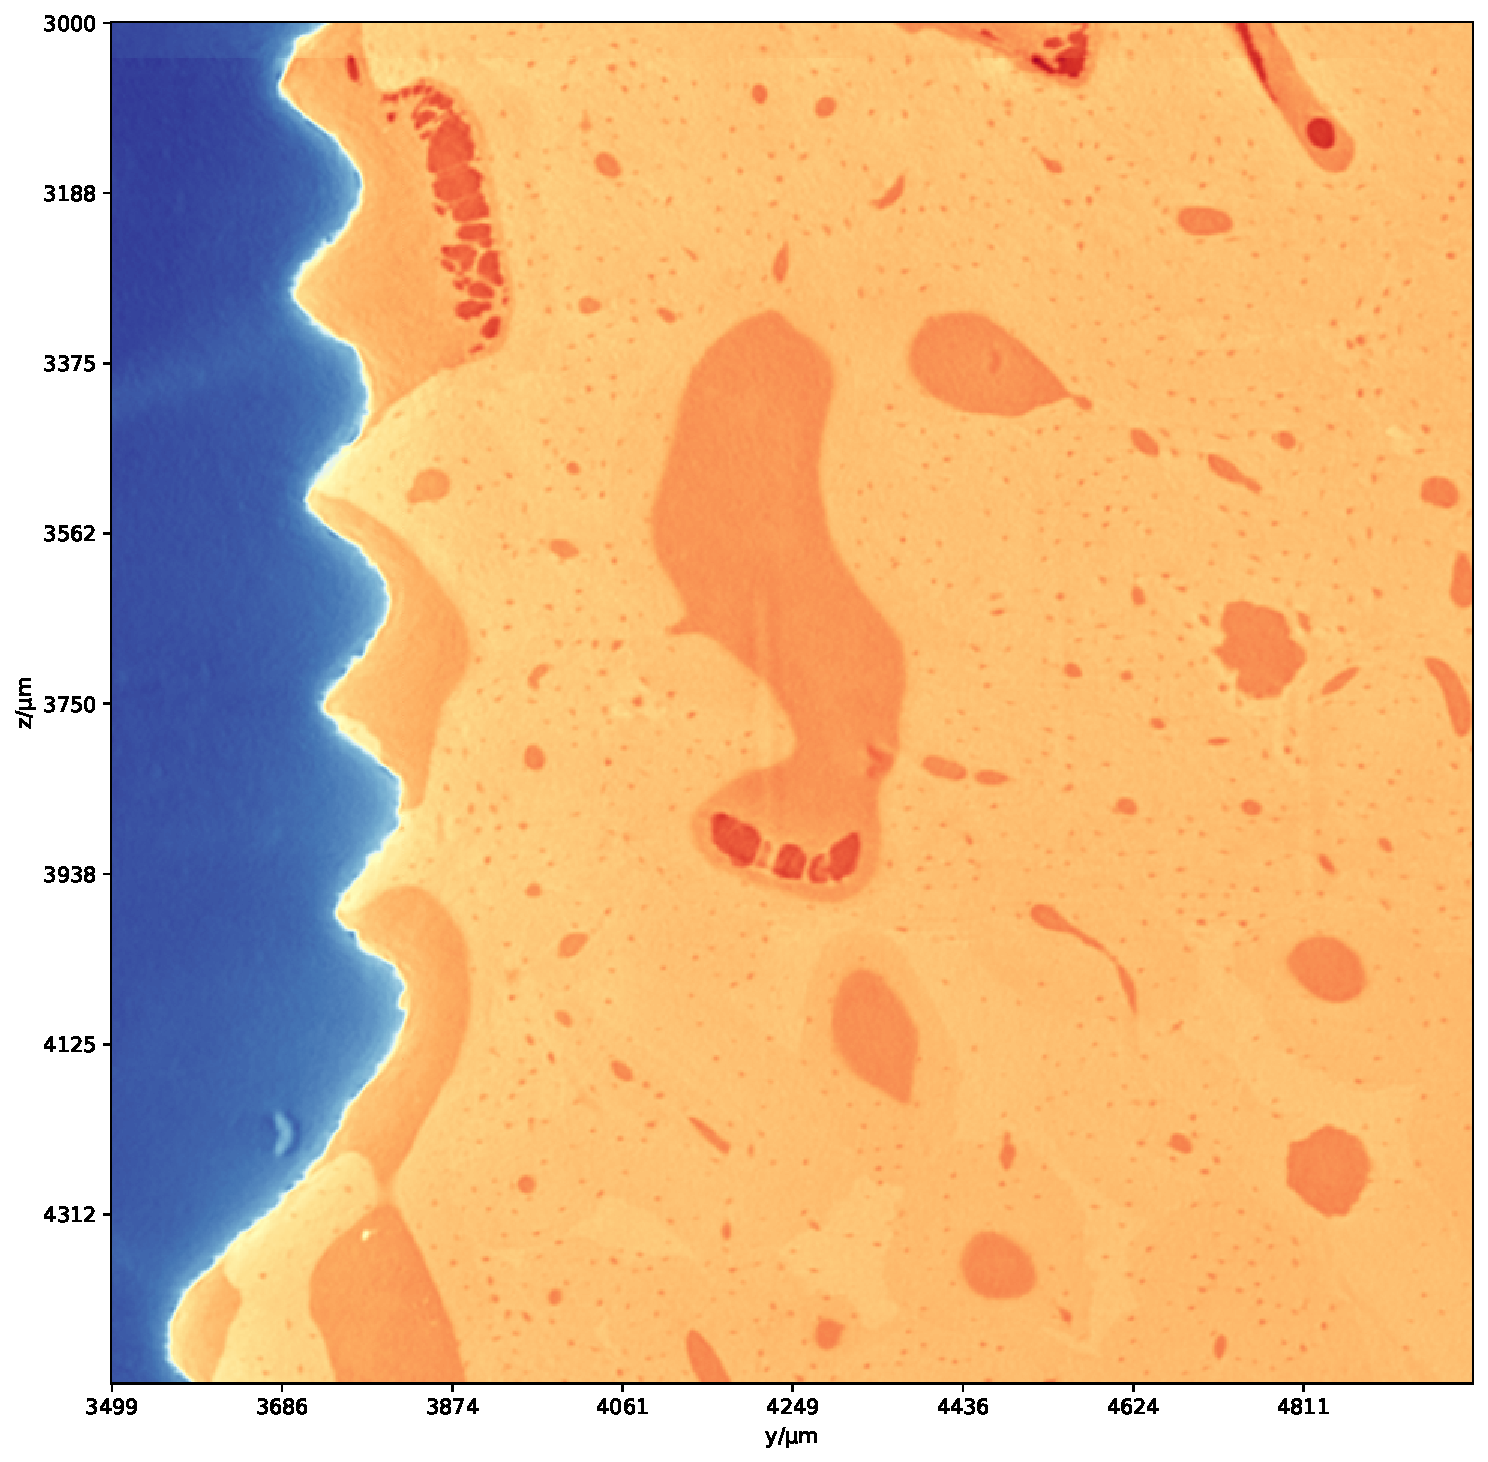
\includegraphics[width=\linewidth]{generated/770c_pag_segmented_zy_raw.pdf}
      \caption{Tomographic slice}
    \end{subfigure}%
    \begin{subfigure}{0.5\textwidth}
      \centering
      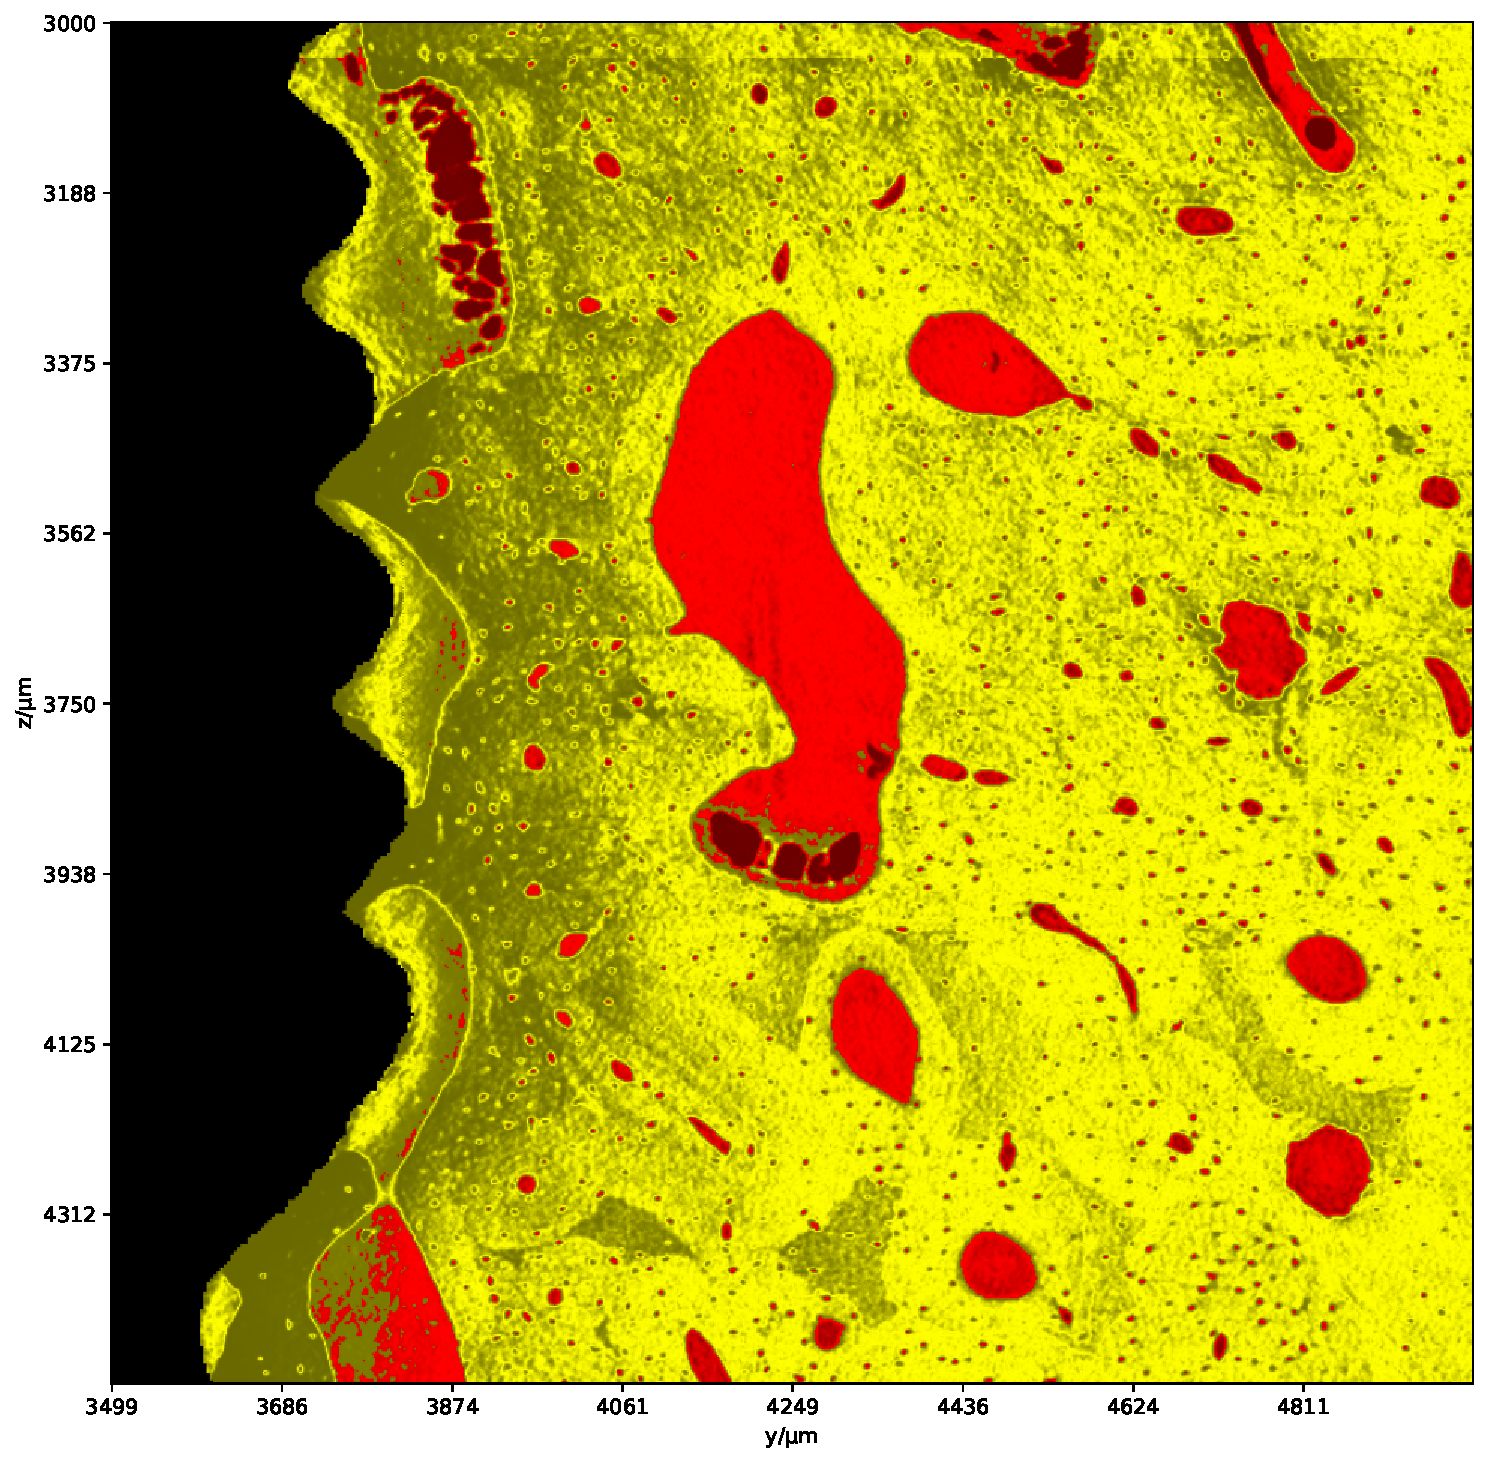
\includegraphics[width=\linewidth]{generated/770c_pag_global_zy.pdf}
      \caption{Global threshold}
    \end{subfigure}
    \\
    \begin{subfigure}{0.5\textwidth}
      \centering
      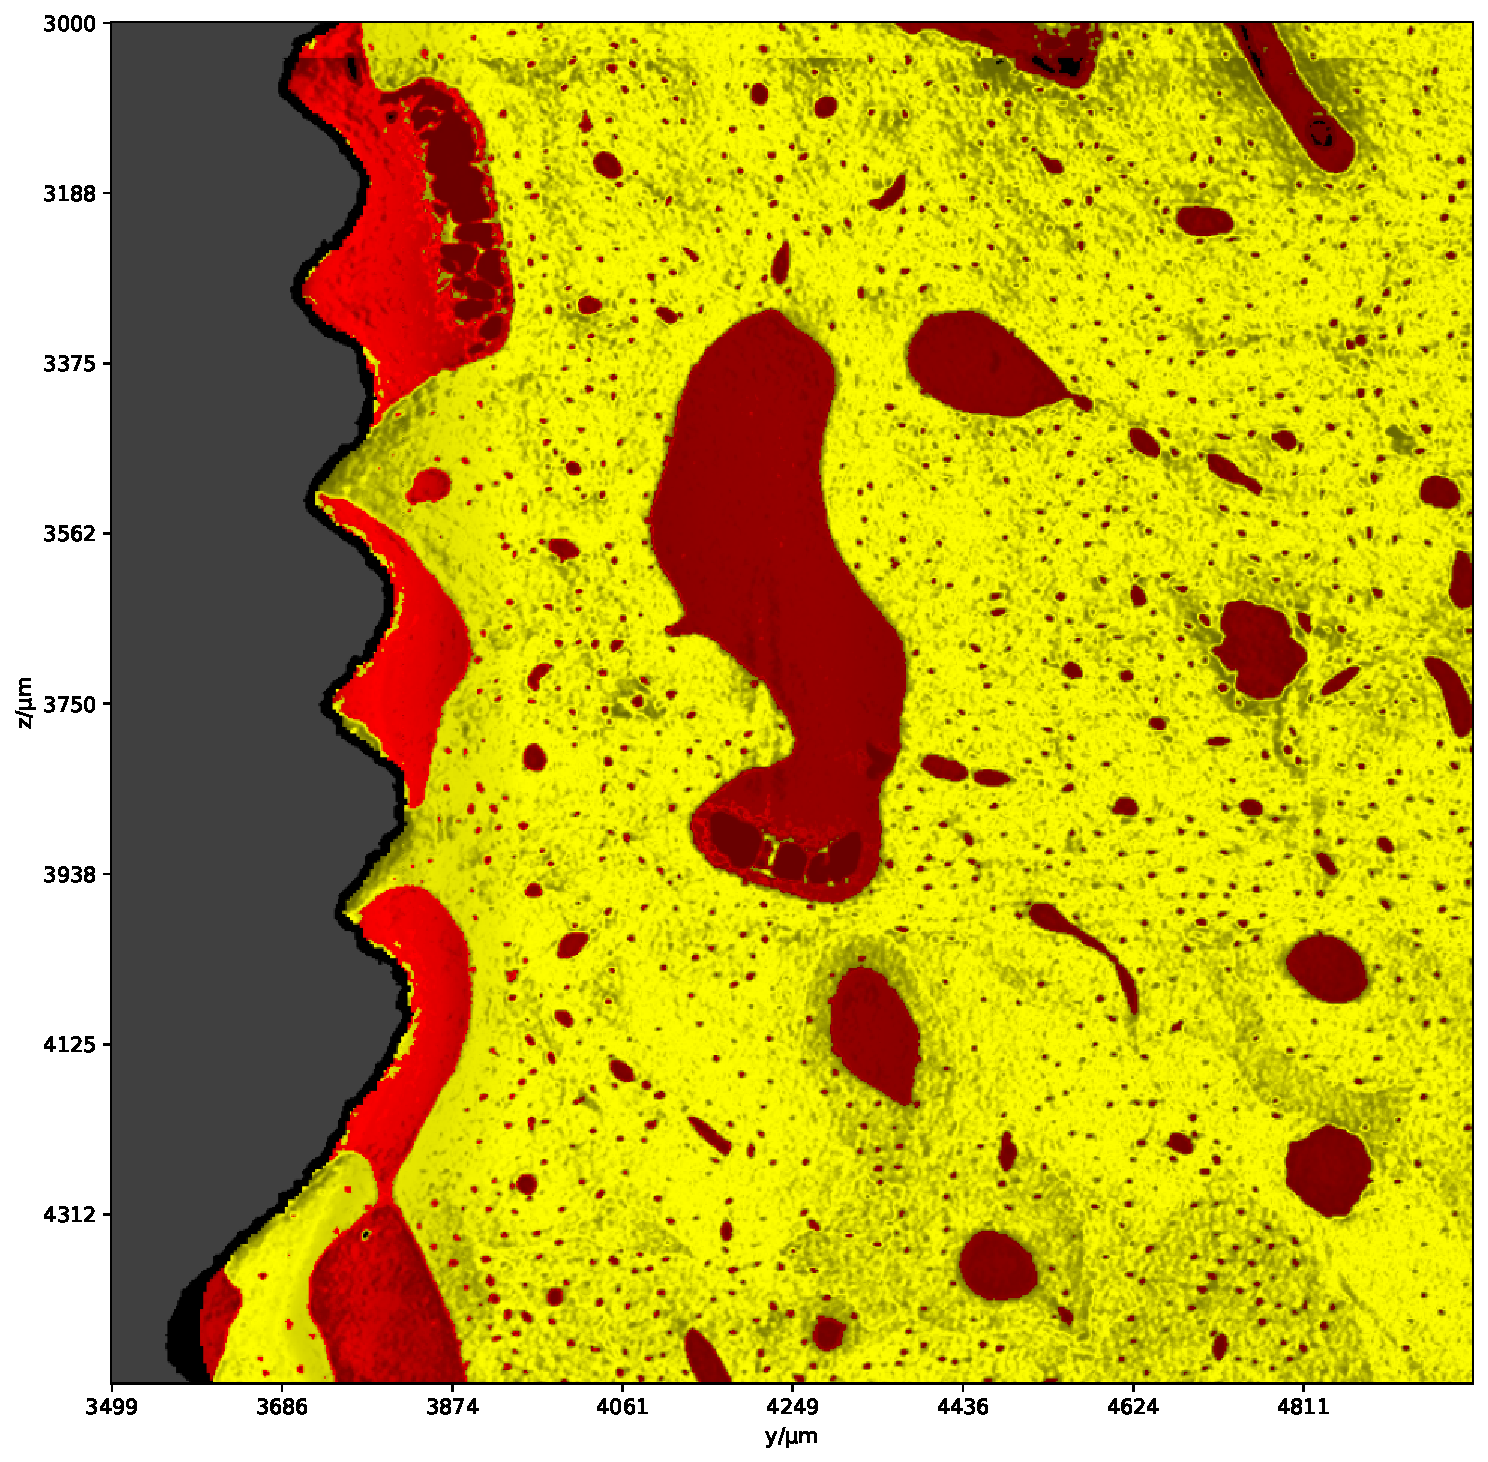
\includegraphics[width=\linewidth]{generated/770c_pag_segmented_zy_colored.pdf}
      \caption{SASS}
    \end{subfigure}%
    \begin{subfigure}{0.5\textwidth}
      \centering
      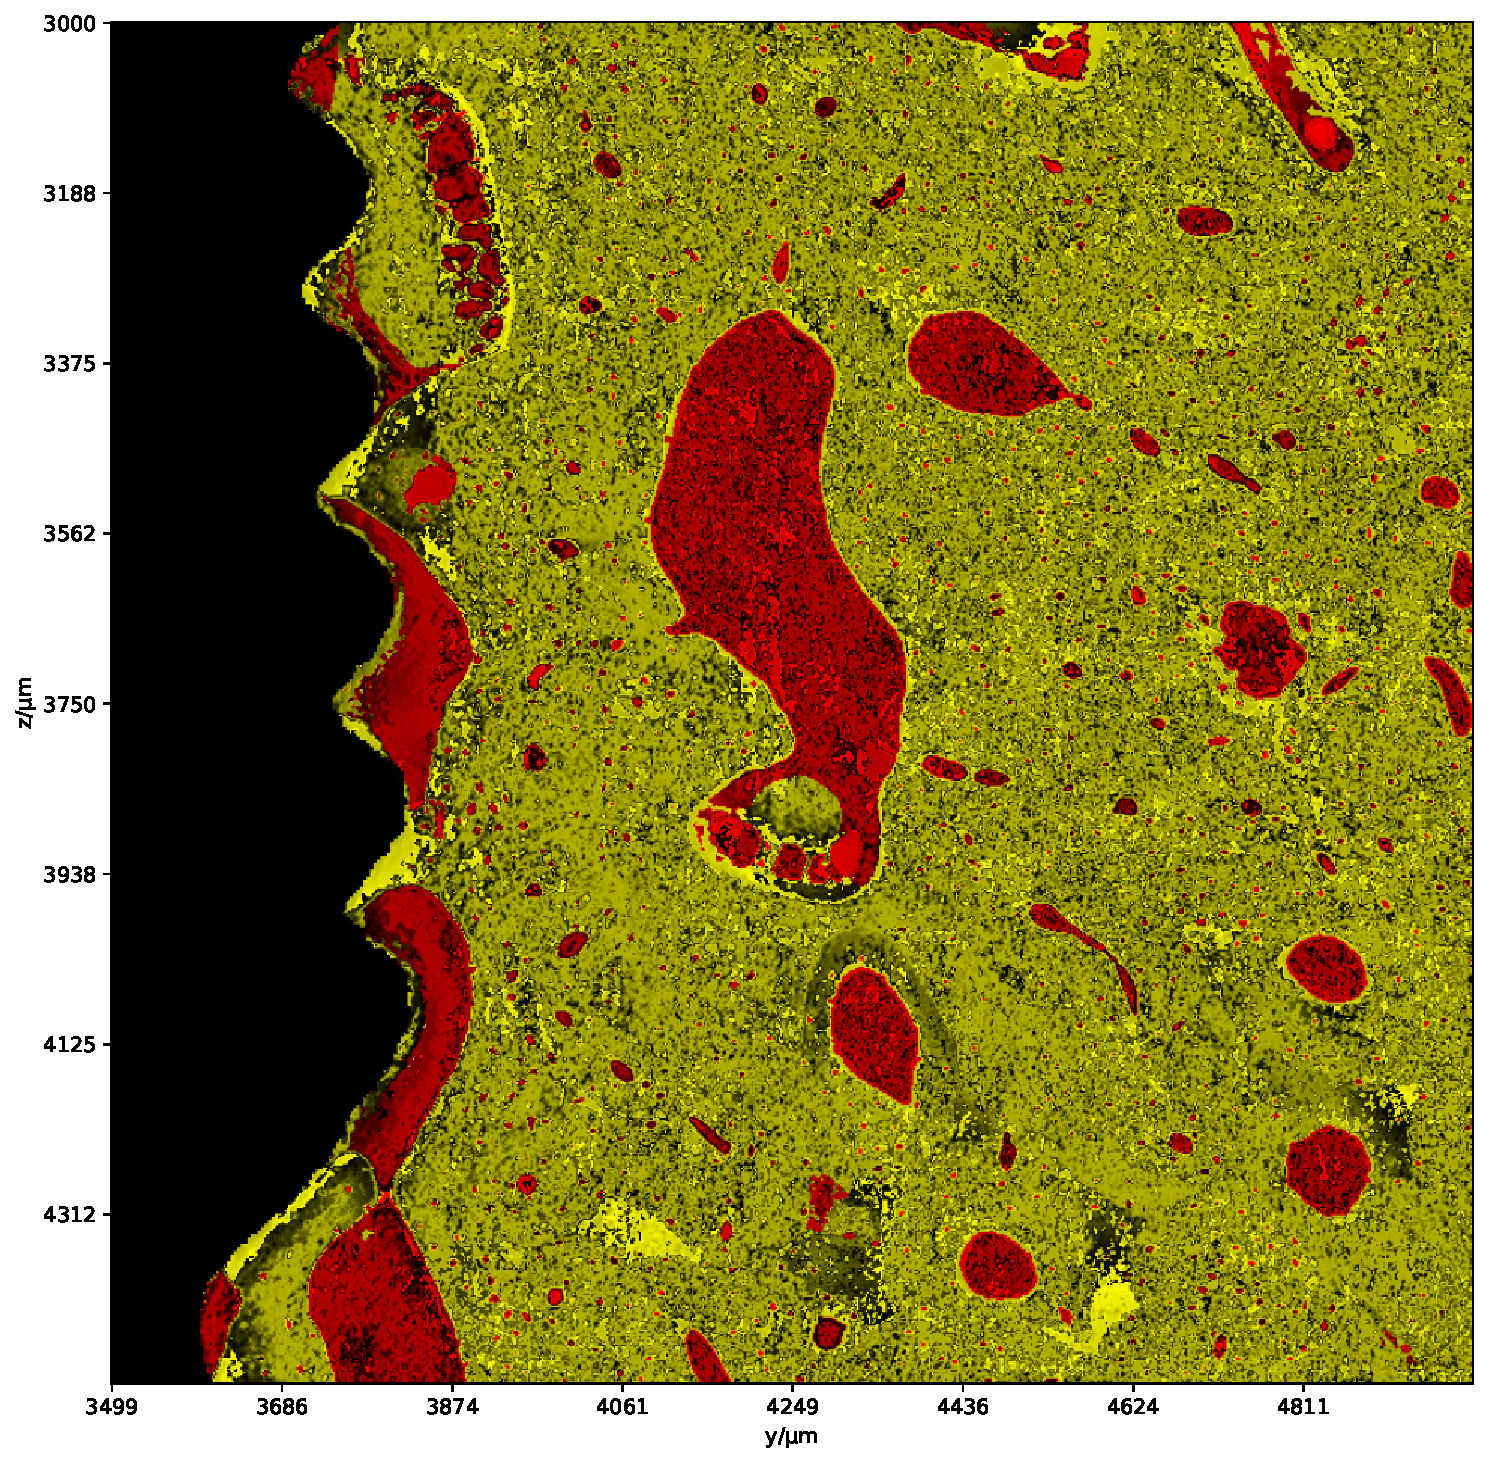
\includegraphics[width=\linewidth]{generated/770c_pag_global_zy_otsu.pdf}
      \caption{Adaptive Otsu}
    \end{subfigure}
  \caption{
	  YZ-slices of the original tomography, global threshold segmentation,
	  SASS and adaptive Otsu segmentation. Yellow depicts bone and red
	  depicts soft tissue. Note that SASS correctly classifies the
	  materials close to the implant, and particularly in the grooves of
	  the screw threads, whereas the global threshold and adaptive Otsu
	  segmentation fails.
    }
    \label{fig:histology-comparison2}
\end{figure*}

We see that SASS is overall successful in identifying actual features, rather
than artifacts, and classifying the internal darker regions as soft tissue and
the lighter regions as bone. This is further confirmed in
\Cref{sec:blood-network}. However, extremely close to the implant (a few
voxels), we cannot verify the segmentation, as the voxel values are so blended
together with the implant voxel values that they become indistinguishable. A
further strengthening of the analysis is needed to reach this layer. It is
possible that the information is irretrievably lost, or perhaps it can be
retrieved through a different method, such as deconvolution.  It also fails
within some soft tissue blobs, which is due to air bubbles in the resin, which
have a very low density and therefore a very low absorption.

\subsection{Quantitative evaluation}

% Why it is a problem
Reliably evaluating segmentation methods on medical data such as that
presented in this paper is a challenging task. A satisfactory annotated ground
truth does not exist, which makes quantitatively evaluating one method against
another very hard. Furthermore, due to the very large number of voxels, using
manual or semi-automatic methods quickly becomes impractical. One such example
are neural networks, which need to be trained on multiple instances of similar
data accompanied by an annotated ground truth. This is a very time-consuming
and expensive procedure, and does not easily translate to other data, which are
only slightly dissimilar.

% How are we going to approach it
To ensure a reliable and consistent verification of the presented SASS method,
we must tackle the common replication problem~\cite{replication-crisis} where
solutions are often hard to reproduce and therefore verify. Furthermore, many
existing evaluation procedures involve comparing results to manual
segmentations performed by a human~\cite{seg_literature_review}. We attempt to
overcome these difficulties by creating synthetic reproducible data,
accompanied by a consistent reference level ground truth. The generated data
resembles our original data and shares many physical qualities, but instead of
being acquired at ESRF, it is simulated using the software
Novi-sim~\cite{novisim} on a consumer-grade workstation. It is therefore not
realistic to expect the quality of the simulated tomograms to be identical to
real data. It is more important that it captures the expected spatial
distributions of noise and thereby resembling the real data well enough to use
for validation.  Using such simulations allow other researchers to not only
reproduce but also modify our tomographic models and perform new experiments.
This will both extend the robustness of SASS, and make it less specific and
dependent on our original data.  In future experiments this also allows
extracting 2D-slices of synthetic data and compare with manually inspected and
annotated histologies.

\begin{figure*}
  \centering
  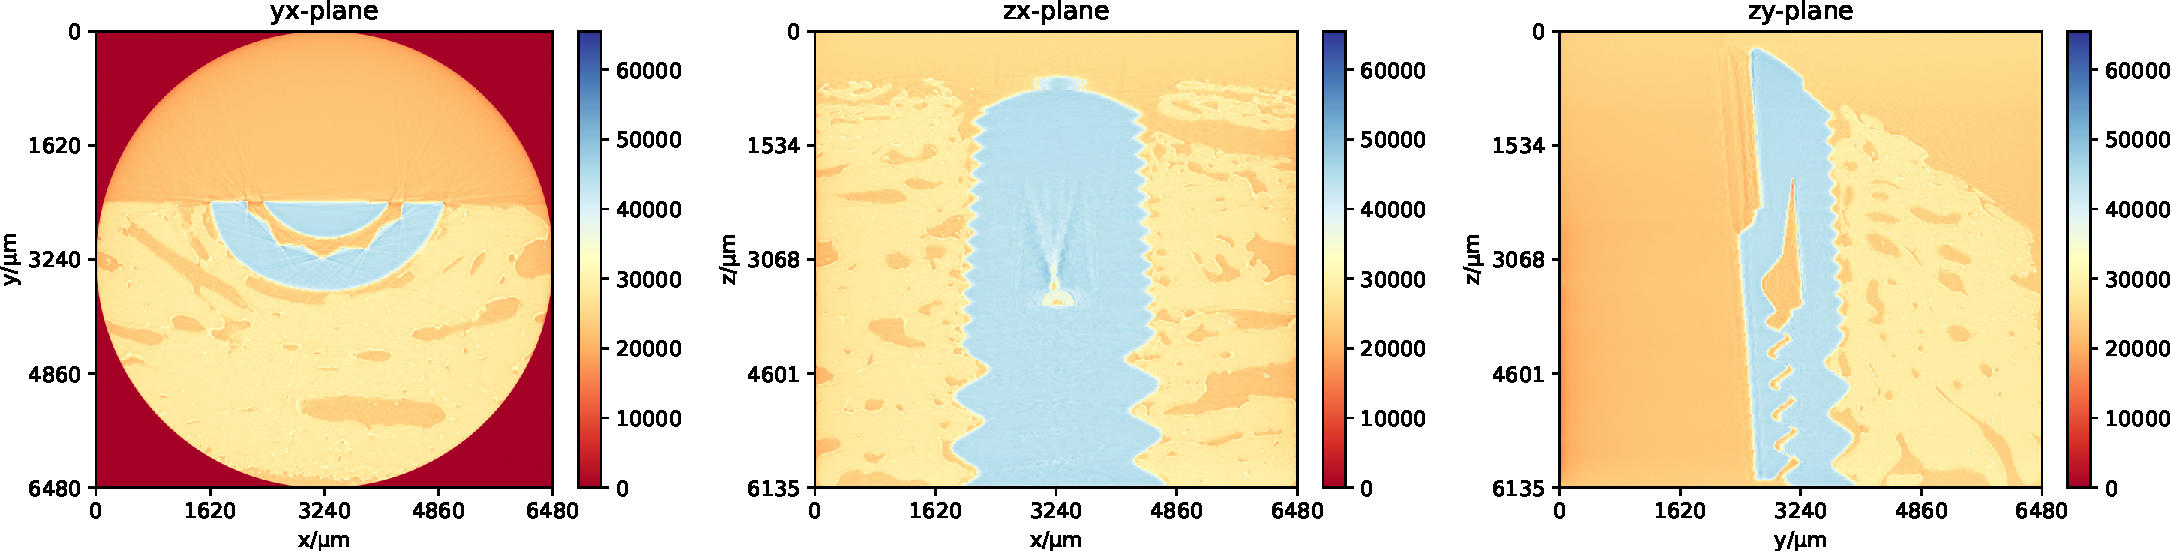
\includegraphics[width=\textwidth]{figures/novisim_raw_2x.pdf}
  \caption{Simulated tomogram from Novisim. This is ideally comparable to the
	true data as shown in \cref{fig:3viewsample}. We do notice that the
	numerical ranges are offset relative to \cref{fig:3viewsample}, but the
	ordering is naturally the same.}
  \label{fig:novisimraw}
\end{figure*}

\subsection{Ground truth and synthetic data}

% How we use Novi-sim
The presented segmentation pipeline results in a set of masks, one for each
material. Each mask is overlayed unto a single volume forming what we define as
our artificial ground truth. By construction, it will have a perfect overlap,
correctly identifying each material using the SASS method on real sample data.
The masks for each material are converted into meshes and used to generate STL
files.  The generated STL files are used to simulate synthetic tomograms using
Novi-sim. We unfortunately had no luck using the full resolution scaling with
our STL models, so we ended up using a 4x downscale. This will of course remove
the finest features in the simulated tomograms, but the overall quality remains
good. While the software is set up to resemble the original experiment at ESRF,
it is not reasonable to expect a perfect match. The defined ground truth is by
design perfectly accurate with respect to the SASS segmentation output on real
data, but deviates predictably from the simulated tomogram data due to
experimental physical effects and scattering artifacts. This now allows us to
use our reproducible synthetic data to consistently compare the SASS method
with other approaches and detect in which regions they differ the most. Because
regions very close and very far away from the implant are difficult, any
intermediate regions should be fairly consistent across methods.  Finally, we
can inspect the differing regions visually to evaluate on the overall
performance. This results in a drastically reduced volume needed to be manually
inspected.

The segmented volumes are evaluated as a function of the distance from the
implant. We inspect regions at short, mid and long radial distances from the
implant. This is shown in \Cref{tab:scores}. To ensure a fair comparison, both
global and adaptive Otsu thresholding is computed on individual slices through the depth
of the implant. The scores for all slices are then averaged for each evaluation
metric, and it is the average value which is reported in \Cref{tab:scores}.
This procedure serves to remove any bias of choosing specific regions where one
approach might falsely appear superior.

\begin{figure*}
  \centering
  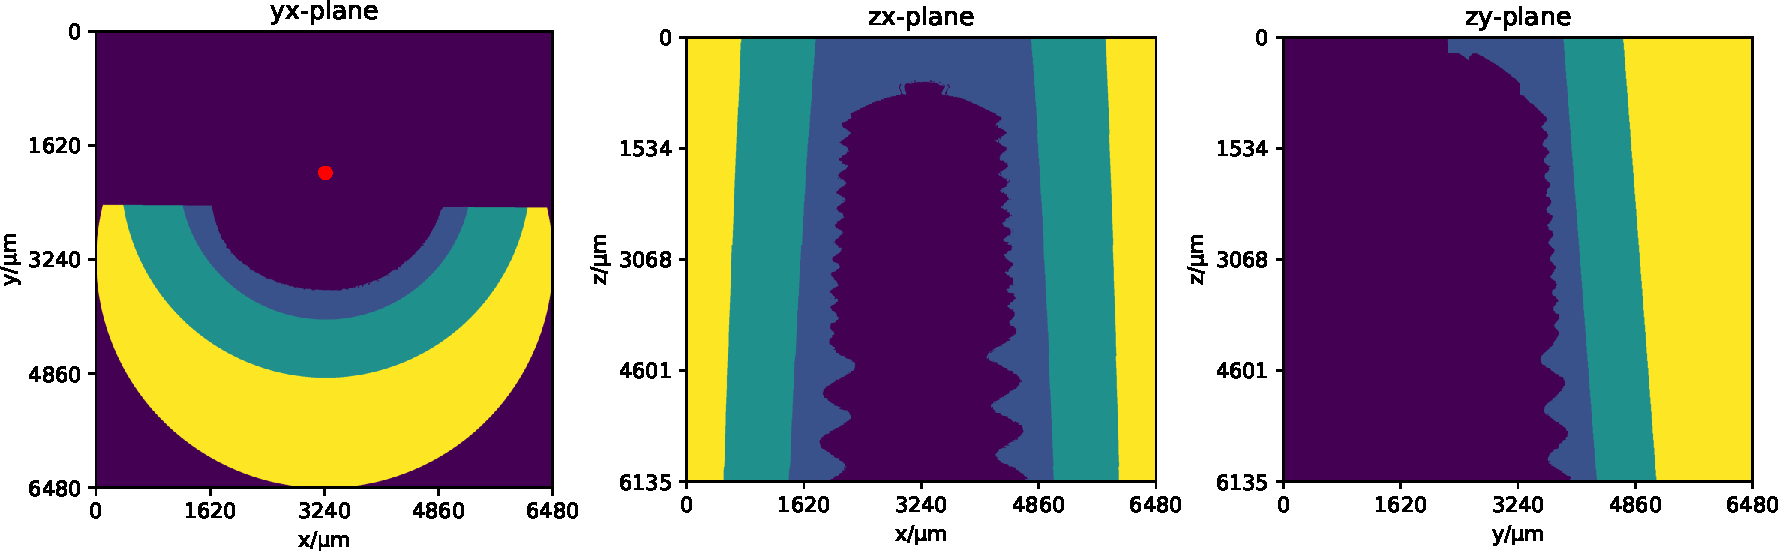
\includegraphics[width=\textwidth]{figures/radial_masks.pdf}
  \caption{Three radial masks are computed, representing short, mid and
	long range distance regions away from the implant. The red dot marks
	the true implant center, which does not coincice with the cut cylinder
	center. It is the true implant center which is used as the radial
	center for the masks. The implant and irrelevant regions containing air
	are removed.  These radial masks are then used for evaluation at
	various distances as a function of the implant radius.
	\cref{tab:scores}.}
  \label{fig:radialmasks}
\end{figure*}

\begin{table*}[]
\caption{
	Classification scores of studied segmentation methods on simulated
	tomograms relative to ground truth, showing different aspects of
	similarity. DS refers to the Dice-Sørensen coefficient, MSE is the Mean
	Squared Error and VOE is the Volumetric Overlap Error. Instead of just
	looking at the BIC close to the implant, we evaluate the overall
	quality of the segmentation as a function of the distance from the
	implant. The distance is reported as a fraction of the implant radius.
        }
\label{tab:scores}
\centering
\begin{tabular}{lccc}
 & \shortstack{DS \\ (blood, bone)} & \shortstack{MSE \\ (blood, bone)} & \shortstack{VOE \\ (blood, bone)}\\
\toprule
$d \leq 0.25 \times R$ (\textbf{Short range}) & & &  \\
\midrule
Global threshold & (0.6273, 0.7807) & (0.0113, 0.0134) & (0.0543, 0.3597) \\
Adaptive Otsu    & (0.7159, 0.8599) & (0.0963, 0.0880) & (0.4425, 0.2458) \\
SASS             & (0.9322, 0.9246) & (0.0027, 0.0038) & (0.1270, 0.1402) \\
\toprule
$ 0.25 \times R < d < 0.50 \times R$ (\textbf{Mid range}) & & & \\
\midrule
Global threshold & (0.7981, 0.9190) & (0.0103, 0.0148) & (0.3360, 0.1498) \\
Adaptive Otsu    & (0.8562, 0.9426) & (0.0886, 0.1010) & (0.2514, 0.1085) \\
SASS             & (0.9267, 0.9551) & (0.0044, 0.0078) & (0.1366, 0.0860) \\
\toprule
$d \geq 0.50 \times R$ (\textbf{Long range}) & & & \\
\midrule
Global threshold & (0.8498, 0.9489) & (0.0090, 0.0149) & (0.2611, 0.0973) \\
Adaptive Otsu    & (0.8562, 0.9514) & (0.0959, 0.1181) & (0.2514, 0.0927) \\
SASS             & (0.8421, 0.9481) & (0.0105, 0.0148) & (0.2727, 0.0987) \\
\bottomrule
\end{tabular}
\end{table*}

\Cref{tab:scores} shows all classification scores for implant, bone and blood
masks respectively, for all studied segmentation methods. We report three
different evaluation scores. The Dice-Sørensen (DS) coefficient measures the
similarity of two volumes based on their overlap, where 1 means perfect overlap
and 0 means no overlap. The valid range is $[0,1]$. The MSE squares the error
such that positive and negative deviations are treated equally, and larger
deviations contribute more to the resulting error. The error is divided by the
total number of voxels in a volume, making the MSE comparable between volumes
of different size.  The valid range is $[0,\inf]$. The VOE measures the
dissimilarity of two volumes based on how much the union of two sets differs
from their intersection. Here 0 means perfect overlap and 1 means no overlap.
The valid range is $[0,1]$.

The DS is very commonly used~\cite{evaluation_review}, and intuitive to
interpret as a simple percentage of overlap between the two sets. The VOE
differs from the DS score by how overlapping voxels are accounted for, and is
thus more sensitive to small differences in overlap. This can make it more
intuitive for comparing high-resolution segmentations.

We see in \Cref{tab:scores} that the SASS method generally outperforms global
and adaptive Otsu thresholding. The difference is largest for the blood
networks, which makes sense because they are also the most difficult. One
region towards the top of the implant adds significantly to the error of all
segmentation methods. This region is located towards the top part of the
implant, for example shown in the zx- and zy-planes in \cref{fig:radialmasks}.
If we manually choose to ignore this region, all three metrics will be
improved. This is however handpicking regions, and outside the scope of this
work, geared towards a fully automated approach. We also note that our MSE is
the smallest in all cases, and often by an order of magnitude. In all cases,
the dominating contribution to error arrise from edge effects at the outer
edges of the cylinder. Here our model lacks sufficient amounts of data voxels
to properly create reasonable probability distributions for all present
materials. If we shave off the outermost layer of voxels, this error is
reduced. While our method can be improved by adding more information to our
composite model, this is left for, and described in future work.

% TODO (James): Omdøb/ryk nedenstående subsection "Dataset analysis" til mere
% passende navn/sted Det er jo egentlig mere motivation og application osv.  De
% to subsubsections "Blood vessel network" + "Implant contact" skal også
% omdøbes/rykkes

\subsection{Dataset analysis}

Having verified the method qualitatively and quantitatively, we can have a more
detailed look into the segmented data. We are interested in the blood vessel
network in the bone region and the tissue-to-implant contact. We will start by
analyzing the blood vessel network and then the tissue-to-implant contact.

\subsubsection{Blood vessel network}
\label{sec:blood-network}

With a good separation of soft tissue and bone, we map out the blood vessel
network using connected components analysis, which is visualized in the 3D
renders in~\Cref{fig:blood-network}. Here we see that we have successfully
segmented the blood vessels out of the bone region. It is especially prominent
when looking at the capillary network, as we can see these in fine detail.
Noteworthy, the newly formed bone region (\Cref{fig:blood-new-slice}) contains
larger concentrations of small blood vessels, compared to the old bone
(\Cref{fig:blood-old-slice}). If we zoom in on a small cube region
(\Cref{fig:blood-old-cube} and \Cref{fig:blood-new-cube}), we see it even more
defined, clearly seeing how the larger vessels connect through the smaller
ones.

\begin{figure}
    \centering
    \begin{subfigure}[b]{\linewidth}
    \centering
        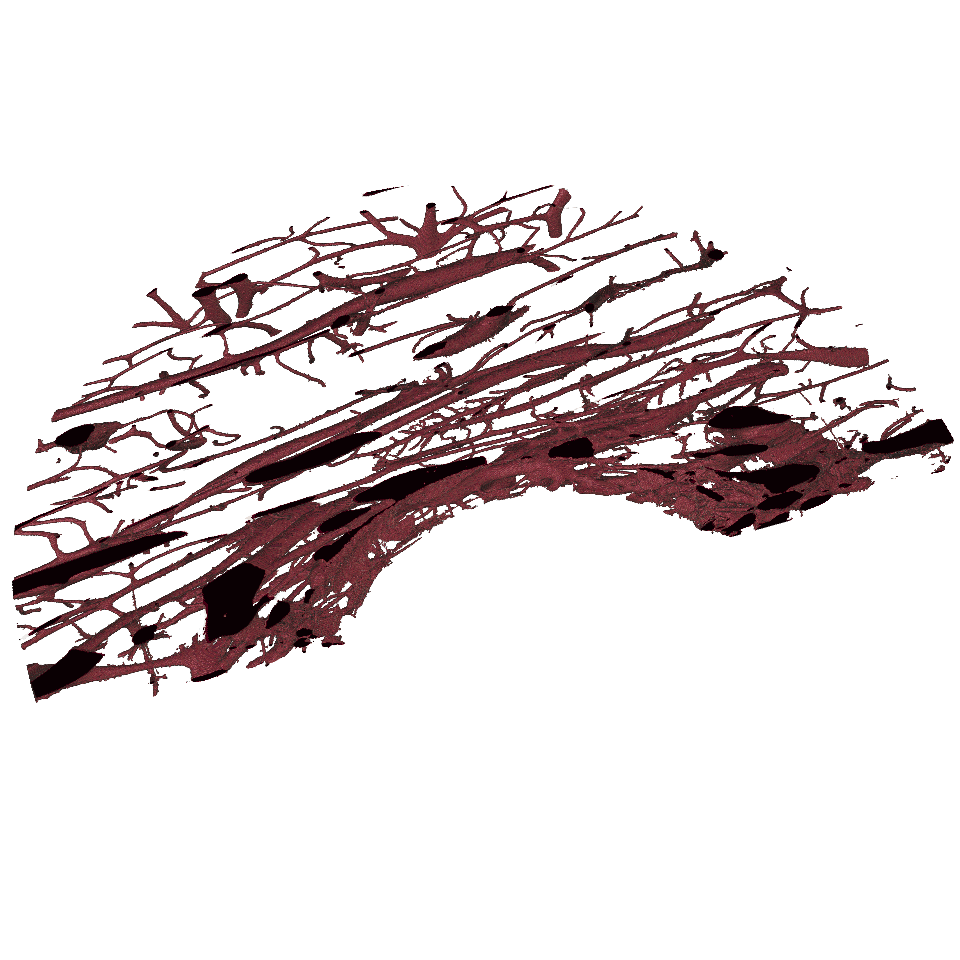
\includegraphics[width=.7\linewidth]{generated/figure10_old_bone.png}
        \caption{A 375 µm $\times$ 4230 µm $\times$ 6480 µm slice of the blood network in the old bone region.}
        \label{fig:blood-old-slice}
    \end{subfigure}
    \begin{subfigure}[b]{\linewidth}
    \centering
        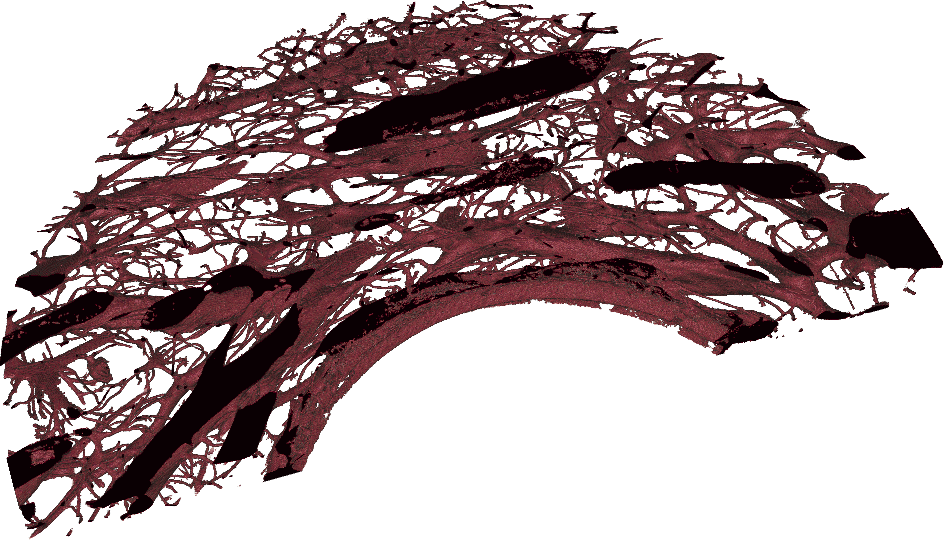
\includegraphics[width=.7\linewidth]{generated/figure10_new_bone.png}
        \caption{A 375 µm $\times$ 4230 µm $\times$ 6480 µm slice of the blood network in the new bone region.}
        \label{fig:blood-new-slice}
    \end{subfigure}
    \begin{subfigure}[b]{.48\linewidth}
    \centering
        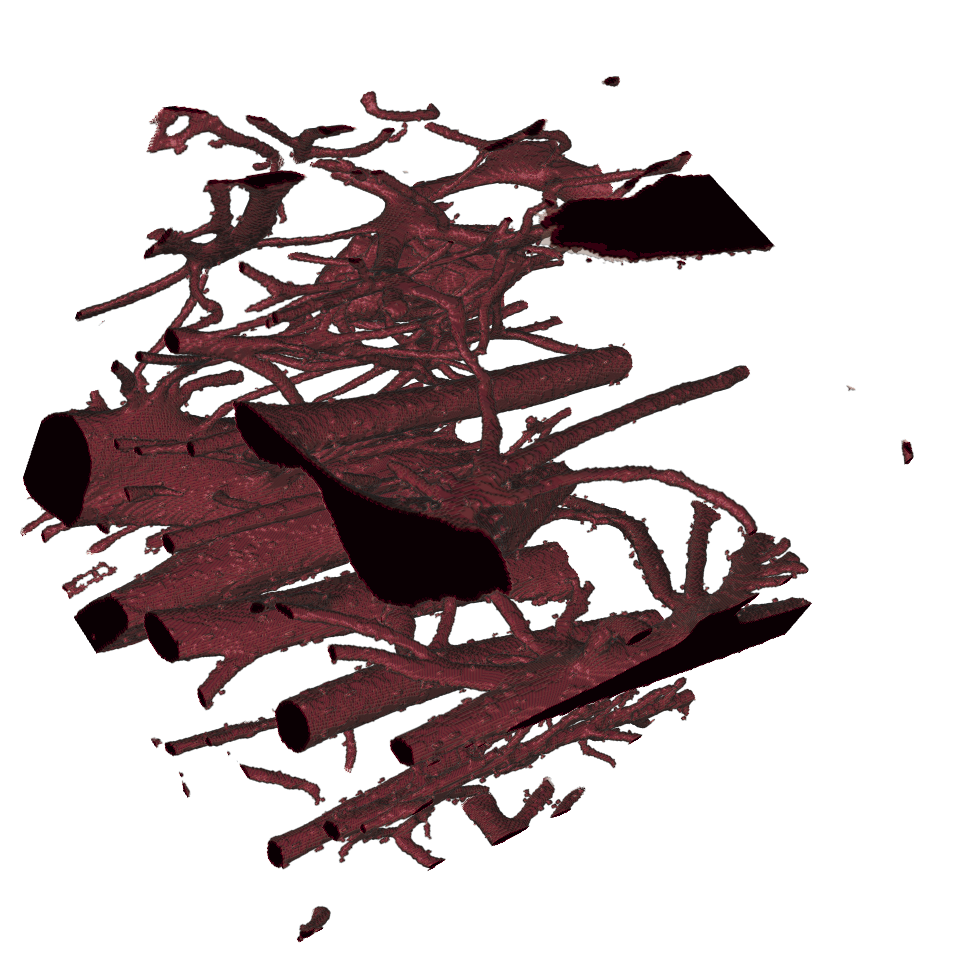
\includegraphics[width=.9\linewidth,height=\linewidth]{generated/figure10_old_cube.png}
        \caption{A $1mm \times 1 mm \times 1 mm$ cube of the blood network in the old bone region.}
        \label{fig:blood-old-cube}
    \end{subfigure}
    \hfill
    \begin{subfigure}[b]{.48\linewidth}
    \centering
        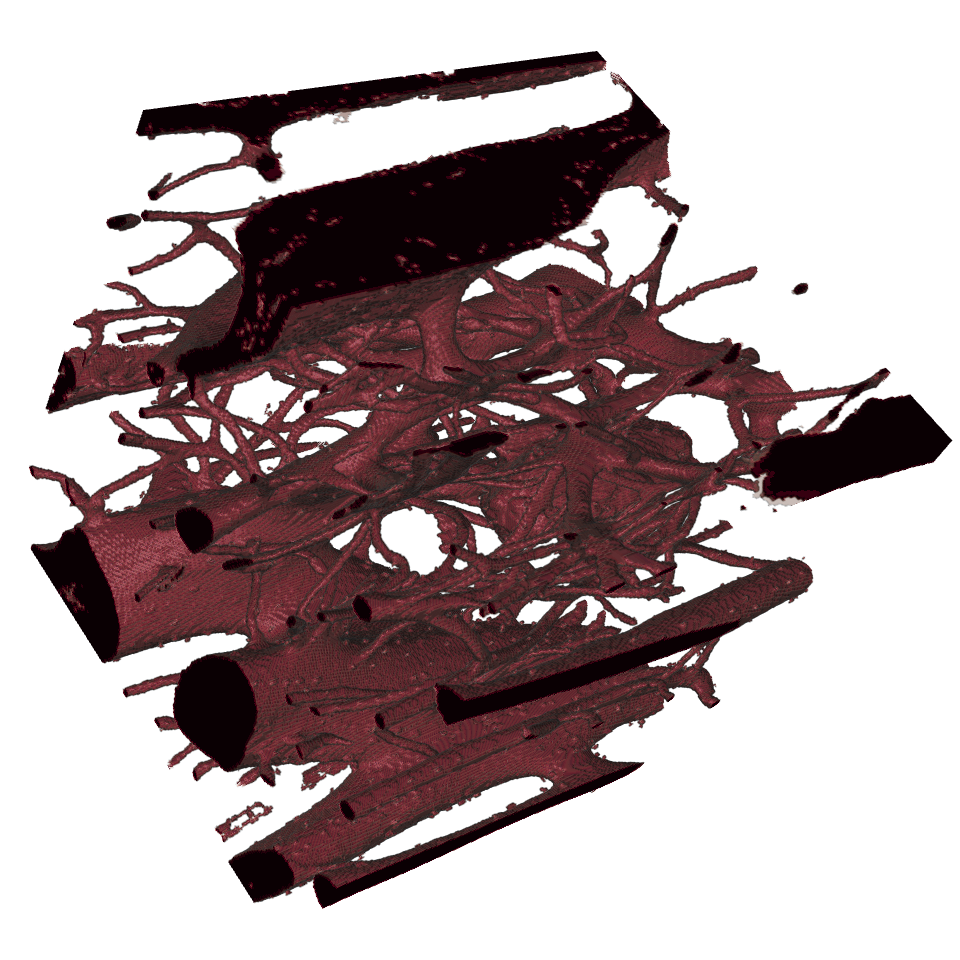
\includegraphics[width=.9\linewidth,height=\linewidth]{generated/figure10_new_cube.png}
        \caption{A $1mm \times 1 mm \times 1 mm$ cube of the blood network in the new bone region.}
        \label{fig:blood-new-cube}
    \end{subfigure}
    \caption{
        3D renders of the blood network. We see a difference between the
        capillary network in the old bone region
        (\ref{fig:blood-old-slice},\ref{fig:blood-old-cube}) compared to the
        newly grown bone region
        (\ref{fig:blood-new-slice},\ref{fig:blood-new-cube}), where the new
        bone region contains a higher concentration of small blood vessels,
        compared to the old bone region containing fewer larger blood vessels.
    }
    \label{fig:blood-network}
\end{figure}

\subsubsection{Implant contact}
\label{sec:contact}

Tissue in contact with the implant can be studied using the EDT from the
implant, restricted to the bone region. We can simply mask the voxels that are
within a thin shell of distances, $d_{min} < d(x,y,z) \le d_{max}$, for
example, $d_{min} = 1 \text{µm}$ to $d_{max} = 5 \text{µm}$. We then sum over
the masked voxels of each tissue type to obtain and divide by the total to
obtain the tissue-to-implant contact per area or study the distribution across
the surface area qualitatively. In particular, we are interested in the
difference between the old and new bone regions. We define the metric as
follows:

\begin{equation}
    BIC = \frac{\sum_{i : \text{field}(i) < 5} \text{bone}(i)}{\sum_{i : \text{field}(i) < 5} \text{voxels}(i)}
\end{equation}

% TODO (James): Bør vi præcisere hvordan ny/gammel region er fundet? Vi bruger
% IKKE en automatisk metode, men har håndholdte værdier til at definere
% overgangen mellem små og store threads. Ikke desto mindre, er det ikke særligt
% detaljeret forklaret her. Måske er det OK. Lidt voldsomt at lave plots for dette.
We find the old and new bone regions at different $z$ levels, based on the
threading of the implant, with new bone being near the small threads and old
bone being near the large threads. The results can be seen in \Cref{tab:bic}.
We see that the BIC is higher in the old bone region than in the new bone
region, which is expected as the bone grows around the implant over time. This
is further confirmed by the blood vessel network analysis as seen in
\cref{fig:blood-network}, as the new bone region contains a higher
concentration of small blood vessels, indicating that the bone is still
growing. This shows that the method is successful in segmenting the bone and
soft tissue regions and that the segmentation can be used to study BIC.

\begin{table}
    \caption{The mean and standard deviation of bone-to-implant contact in the
    old and new bone regions for each of our samples.}
    \label{tab:bic}
    \centering
    \begin{tabular}{lcc}
        \toprule
        Sample & Old bone & New bone \\
        \midrule
	% TODO: James: Comment in caption why 770 has no new bone numbers
        770 & $0.5020 \pm 0.1222$ & - \\
        770c & $0.6519 \pm 0.1055$ & $0.5638 \pm 0.0907$ \\
        771c & $0.4517 \pm 0.1708$ & $0.5016 \pm 0.1078$ \\
        772 & $0.7012 \pm 0.1065$ & $0.5222 \pm 0.0869$ \\
        775c & $0.2802 \pm 0.0928$ & $0.2652 \pm 0.1054$ \\
        810c & $0.6819 \pm 0.0866$ & $0.5155 \pm 0.0897$ \\
        811 & $0.5832 \pm 0.1015$ & $0.3715 \pm 0.0935$ \\
        \bottomrule
    \end{tabular}
\end{table}

\begin{table}
    \caption{
	    The mean and standard deviation of bone-to-implant contact in the
	    old and new bone regions for the simulation and the original sample
	    in the same resolution as the simulation.
	    }
    \label{tab:bic-sim}
    \centering
    \begin{tabular}{lcc}
        \toprule
        Method & Old bone & New bone \\
        \toprule
	\multicolumn{3}{l}{\textbf{770c\_scaled}} \\
	\midrule
	% TODO: Aleksandar: insert numbers using actual comparable scale
        Global & $0.0 \pm 0.0$ & $0.0 \pm 0.0$ \\
        Adaptive Otsu & $0.0 \pm 0.0$ & $0.0 \pm 0.0$ \\
        SASS & $0.0 \pm 0.0$ & $0.0 \pm 0.0$ \\
	\toprule
	\multicolumn{3}{l}{\textbf{770c\_simulated}} \\
	\midrule
	Global & $0.7523 \pm 0.0403$ & $0.7120 \pm 0.1119$ \\
	Adaptive Otsu & $0.7523 \pm 0.0403$ & $0.7120 \pm 0.1119$ \\
	SASS & $0.7523 \pm 0.0403$ & $0.7120 \pm 0.1119$ \\
        \bottomrule
    \end{tabular}
\end{table}
